\section{Kerndatensatz der \acs{mii}} \label{sec:miikdz}

Einer der Erfolge der \ac{mii} ist, dass alle Mitglieder der \ac{mii} sich auf einen gemeinsamen Kerndatensatz geeinigt haben \cite{telemedizin, miikdz}. Dieser Datensatz ist die wichtigste Voraussetzung für die zentrale Basis für den gemeinsamen Gebrauch von Daten und, dass dieselbe Auswertungslogik in den \acp{diz} lokal ausgeführt werden kann, denn die Daten in der Patientenversorgung stammen heutzutage aus diversen Quellsystemen und liegen somit in vielen verschiedenen Datenformaten mit unterschiedlichem Inhalt vor \cite{miikdz}. 

Mit diesem Kerndatensatz wurde, unabhängig von Use Case und Indikation der Mitglieder der \ac{mii}, festgelegt, welche Datensätze von den stationären und ambulanten Patienten und Patientinnen die \acp{diz} der \ac{mii} mindestens speichern sollten \cite{miikdz}.

Der \ac{mii}-Kerndatensatz besteht aus Basis- und Erweiterungsmodulen (\ref{fig:mii}). Während die Definition der Basismodule fachlich übergreifend ist, sind die Erweiterungsmodule die Abbildung von Daten spezifischer An- wendungs- oder Fachgebiete, sodass der Kerndatensatz in kontinuierlicher Erweiterung ist \cite{miikdz}.

\clearpage

\begin{figure}[ht]
	\centering
	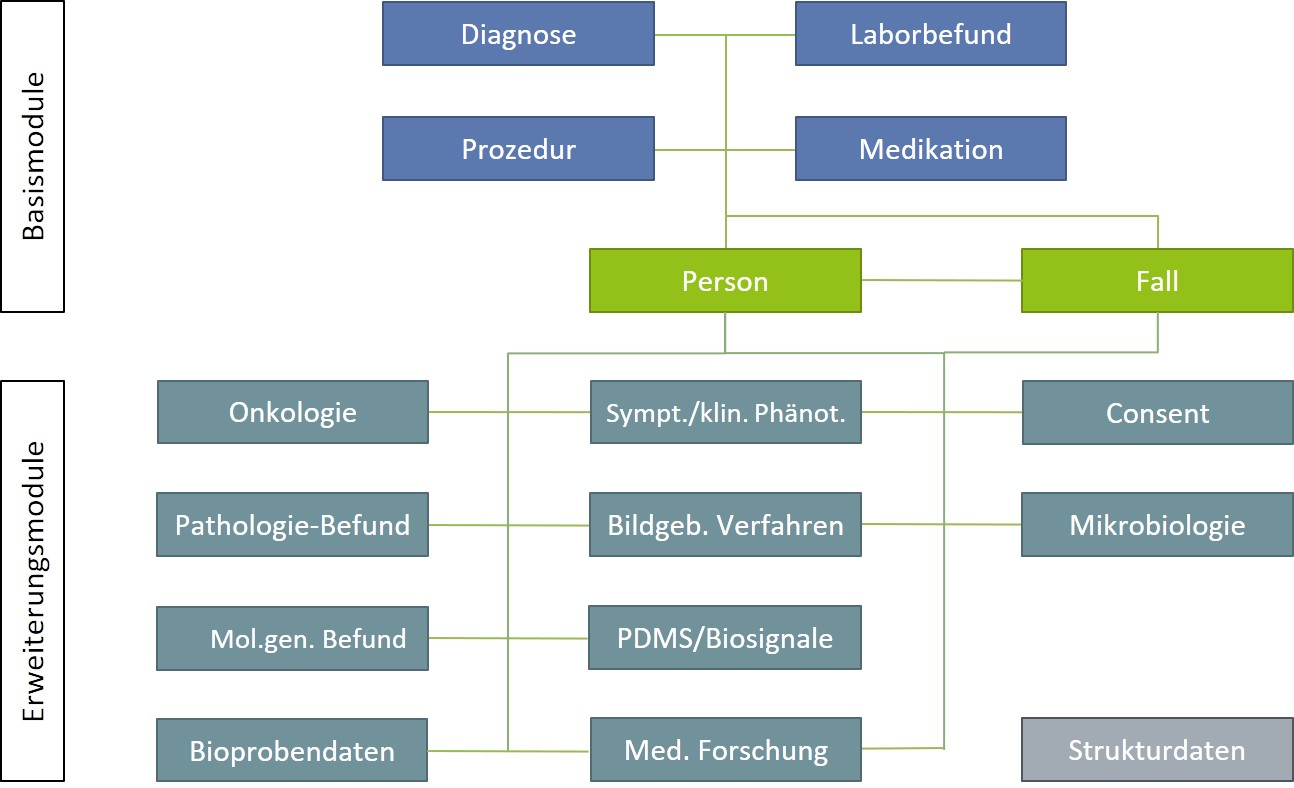
\includegraphics[height=7.5cm]{figures/MIIModule}
	\caption[Kerndatensatz der \acs{mii}]{Kerndatensatz der \acs{mii} und deren Erweiterungsmodule \cite{miikdz}.}
	\label{fig:mii}
\end{figure}

\subsection{Erweiterungsmodul \glqq Intensivmedizin\grqq{} des Kerndatensatzes der \acs{mii}} \label{subsec:icumodul}

Relevant für die Durchführung dieser Masterarbeit ist das Erweiterungsmodul \glqq Intensivmedizin\grqq{} oder \ac{icu}, wie in \ref{fig:mii} als \acs{pdms}/Biosignale genannt. Der Fokus des Projekts liegt ganz konkret auf der \ac{fhir}-Spezifikation des Moduls (\href{https://www.medizininformatik-initiative.de/Kerndatensatz/Modul_Intensivmedizin/IGMIIKDSModulICU.html}{Medizininformatik Initiative - Modul ICU - ImplementationGuide}). Ein wichtiger Hinweis an dieser Stelle ist, dass das Modul \glqq Intensivmedizin\grqq{} auch eine parallele Webseite für die Weiterentwicklung unter der Open Source Plattform SIMPLIFIER.NET (\href{https://simplifier.net/medizininformatikinitiative-modul-intensivmedizin}{Medizininformatik Initiative - Modul ICU}) besitzt, wo die aktuellen Modifikationen veröffentlicht werden. Auf dieser Webseite können die Mitglieder der \ac{mii} und weitere Personen mit Zugang zu dieser Webseite Kommentare und Anmerkungen an die SIMPLIFIER-Webseite des Moduls (\href{https://simplifier.net/MedizininformatikInitiative-Modul-Intensivmedizin/~issues}{Issues}) senden.

Dieses Erweiterungsmodul spezifiziert akutmedizinische Daten für die Primär- und Sekundärnutzung und hat Bezüge zu den Basismodulen (\ref{fig:mii}). Die erste stabile Ballot-Version der \ac{fhir}-Profile des Moduls wurde am 24. Februar 2022 veröffentlicht \cite{modicu}. Ziel der Modellierung dieses Erweiterungsmoduls ist die Datenabbildung der Intensivmedizin und die Darstellung gleichartiger Daten der Notfallmedizin, stationärer und ambulanter Medizin \cite{icukdz}. Ziel des Moduls ist die Unterstützung und Erleichterung der Forschung, Qualitätssicherung, Kommunikation zwischen medizinischen Geräten und der Entscheidungsfindung \cite{modicuvid}.

Das Erweiterungsmodul \glqq Intensivmedizin\grqq{} ist in drei Entwicklungsstufen geplant, davon ist die erste Stufe fertiggestellt, die zweite wurde von 25.02.2022 bis 08.04.2022 zum Abstimmverfahren freigegeben\footnote{Am 07.11.2022 wurde die finale Version des Moduls freigegeben. Dieses Projekt wurde aber mit der ersten stabilen Ballot-Version des Moduls realisiert, welche in Abstimmung war.}, es ist ein Entwurf zur Korrektur und zum Kommentieren; die dritte Stufe befindet sich immer noch in Entwicklung \cite{modicuvid}.

\begin{enumerate}
	\item Entwicklungsstufe 1: Datenmodell
	\item Datenarten der Entwicklungsstufe 2:
	\begin{itemize}
		\item Monitoring und Vitaldaten
		\item Parameter von extrakorporalen Verfahren
		\item Beatmungswerte
	\end{itemize}
	\item Datenarten der Entwicklungsstufe 3:
	\begin{itemize}
		\item Ein-/Ausfuhrbilanzen
		\item Scores
		\item Hochauflösende Daten
		\item Lagerungstherapie
		\item etc.
	\end{itemize}
\end{enumerate}

 Der Schwerpunkt dieses Projekts liegt in den Parametern der Entwicklungsstufe 2 des Moduls. Obwohl der Abstimmungsprozess dieser Stufe abgeschlossen ist, wurde bis jetzt noch keine neue überarbeitete Version der Entwicklungsstufe 2 fertiggestellt.

 Die Datenarten der Stufe 2 besitzen mindestens ein generisches \ac{fhir}-Profil und viele davon auch ein spezifisches Profil, welches wenn möglich verwendet werden sollte \cite{icukdz, modicuvid}. Die generischen Profile modellieren die Daten unabhängig von einer spezifischen Annotation und beschreiben die Struktur für Gruppen von Elementen einer bestimmten Kategorie und sind somit die ersten in der Baumstruktur der \ac{fhir}-Profile (\ref{fig:icutree}) \cite{icukdz}. Die spezifischen \ac{fhir}-Profile hingegen modellieren zusätzlich eine eindeutige semantische Annotation \cite{modicuvid}.
 
 Unter der Gruppe der Parameter von extrakorporalen Verfahren befinden sich die erfassten Daten von \ac{ecmo}-Maschinen, wie die Dauer einer Hämodialysesitzung. In dieser Gruppe werden die gemessenen und eingestellten Werte zusammen mit dem \ac{ecmo}-Gerät erfasst \cite{icukdz}. 
 
 Die Beatmungswerte der Stufe 2 umfassen Daten, wie die Sauerstofffraktion, das Beatmungsvolumen, etc. Der Aufbau dieser \ac{fhir}-Profile ist analog zu Parametern von extrakorporalen Verfahren \cite{icukdz}.

Die \ac{fhir}-Profile unter der Gruppe Monitoring und Vitaldaten umfassen Daten, wie die Herzfrequenz, Körpergröße, die pulsatilen Blutdrücke (systolisch, mittel und diastolisch), etc. Für die pulsatilen Blutdrücke wurde ein weiteres generisches Profil (Blutdruck Generisch) erstellt, um die Kompatibilität mit den deutschen und internationalen Basisprofilen zu gewährleisten \cite{icukdz}. Diese Profile sind auch eine Zusammensetzung von drei separat kodierten \glqq Observations\grqq{}, die dieselben Attribute teilen, nämlich die Spezifikationen für den systolischen, mittleren und diastolischen Blutdruck \cite{icukdz}.

\begin{figure}[ht]
	\centering
	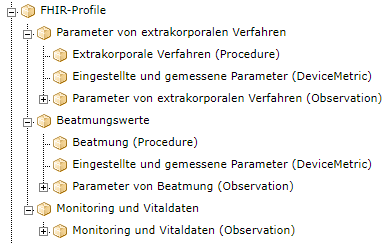
\includegraphics[height=7.5cm]{figures/icu_modul_tree}
	\caption[Baumstruktur des Erweiterungsmoduls \glqq Intensivmedizin\grqq{}]{Baumstruktur des Erweiterungsmoduls \glqq Intensivmedizin\grqq{}.}
	\label{fig:icutree}
\end{figure}

Die semantische Annotation des Erweiterungsmoduls \glqq Intensivmedizin\grqq{} referenziert mindestens einen Primärcode der Terminologie (\ac{snomedct} oder \ac{loinc}) \cite{icukdz, modicuvid}. Um die Interoperabilität mit der Kommunikation zwischen Medizingeräten oder Medizinprodukten zu ermöglichen, wird wenn möglich auch eine semantische Annotation nach \acsu{iso}/\acsu{ieee} 11073-10101\texttrademark{} (\ref{subsec:ieee}) hinzugefügt \cite{icukdz}. Die Maßeinheiten werden nach \ac{ucum} codiert.

\newpage

Die \ac{fhir}-Profile des Moduls \ac{icu} sind in drei Kategorien untergliedert:

\begin{itemize}
	\item DeviceMetric
	\item Observation
	\item Procedure
\end{itemize}

Die \ac{fhir}-Profile der Kategorie \glqq DeviceMetric\grqq{} beschreiben die Messungen und die Einstellungen des benutzten medizinischen Geräts, und sollen wenn möglich mit dem benutzten Gerät verlinkt werden \cite{icukdz}. \glqq DeviceMetric\grqq{}-Profile kategorisieren die Werte in gemessenen und eingestellten Werten \cite{devicemetric}. Die gemessenen Werte sind die während der Untersuchung erhobene Parameter, z. B. die spontane mechanische Atemfrequenz bei der Beatmung. Die eingestellten Werte sind wiederum die Einstellungen an den Geräten, z. B. der eingestellte inspiratorische Gasfluss während der Beatmung.

Die \ac{fhir}-Profile unter der Kategorie \glqq Observation\grqq{} registrieren die Messungen an Patienten, wie Laboruntersuchungen oder die Beobachtungen an Geräten \cite{observation}. Unter dieser Kategorie befinden sich die Vitalparameter.

\glqq Procedure\grqq{}-Profile definieren ein durchgeführtes Verfahren an Patienten, diese können entweder eine physikalische Intervention oder eine Beratung sein \cite{procedure}.
